\documentclass[11pt]{article}

\usepackage[margin=1in]{geometry}
\usepackage{amsmath,amssymb,amsthm}
\usepackage{mathtools}
\usepackage{tikz}
\usepackage{subcaption}
\newtheorem{theorem}{Theorem}
\newtheorem{lemma}{Lemma}
\newtheorem{remark}{Remark}
\definecolor{jobhighlight}{HTML}{9ABCE4}
\newcommand{\machinerow}[2]{%
    \node[machine, anchor=east] at (-0.3,-#1+0.5) {$M_{#2}$};
}

\newcommand{\dotsrow}[1]{%
    \foreach \dy in {-0.18,0,0.18} { % chktex 1
        \fill (-0.6,{-#1+0.5+\dy}) circle[radius=0.025];
        \fill (2,{-#1+0.5+\dy}) circle[radius=0.025];
    }
}

\newcommand{\jobblock}[5][white]{%
    \draw[job, fill=#1] (#3,-#2) rectangle ++(#4,1);
    \node at ({#3 + #4/2},{-#2 + 0.5}) {$#5$}; % chktex 1
}

\newcommand{\schedulethreemaxone}{
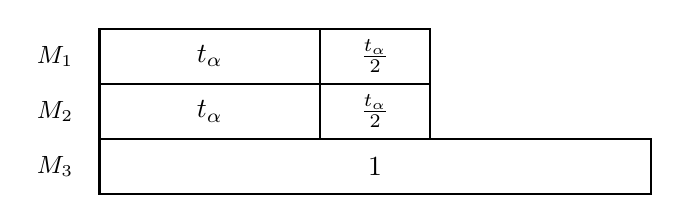
\begin{tikzpicture}[
    x=0.7cm,
    y=0.7cm,
    job/.style={
        draw,
        thick,
        fill=white,
        font=\small
    },
    machine/.style={font=\small}
]

% Displayed machine rows
\machinerow{1}{1}
\machinerow{2}{2}
\machinerow{3}{3}


% Edit the second schedule here.

\jobblock{1}{0}{4}{t_{\alpha}}
\jobblock{1}{4}{2}{\frac{t_{\alpha}}{2}}



\jobblock{2}{0}{4}{t_{\alpha}}
\jobblock{2}{4}{2}{\frac{t_{\alpha}}{2}}

\jobblock{3}{0}{10}{1}
\end{tikzpicture}
}

\newcommand{\schedulethreemaxtwo}{
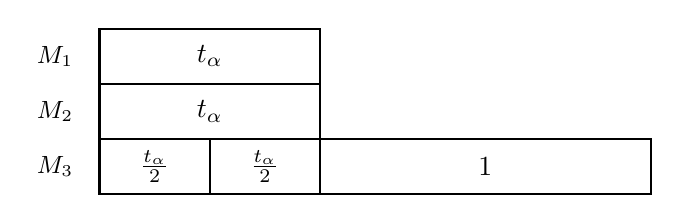
\begin{tikzpicture}[
    x=0.7cm,
    y=0.7cm,
    job/.style={
        draw,
        thick,
        fill=white,
        font=\small
    },
    machine/.style={font=\small}
]

% Displayed machine rows
\machinerow{1}{1}
\machinerow{2}{2}
\machinerow{3}{3}


% Edit the second schedule here.
\jobblock{1}{0}{4}{t_{\alpha}}



\jobblock{2}{0}{4}{t_{\alpha}}

\jobblock{3}{0}{2}{\frac{t_{\alpha}}{2}}
\jobblock{3}{2}{2}{\frac{t_{\alpha}}{2}}

\jobblock{3}{4}{6}{1}

\end{tikzpicture}
}
\newcommand{\schedulethreeone}{
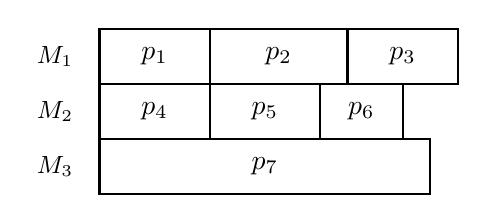
\begin{tikzpicture}[
    x=0.7cm,
    y=0.7cm,
    job/.style={
        draw,
        thick,
        fill=white,
        font=\small
    },
    machine/.style={font=\small}
]

% Displayed machine rows
\machinerow{1}{1}
\machinerow{2}{2}
\machinerow{3}{3}


% Edit the second schedule here.

\jobblock{1}{0}{2}{p_1}
\jobblock{1}{2}{2.5}{p_2}
\jobblock{1}{4.5}{2}{p_3}



\jobblock{2}{0}{2}{p_4}
\jobblock{2}{2}{2}{p_5}
\jobblock{2}{4}{1.5}{p_6}

\jobblock{3}{0}{6}{p_7}
\end{tikzpicture}
}

\newcommand{\schedulethreetwo}{
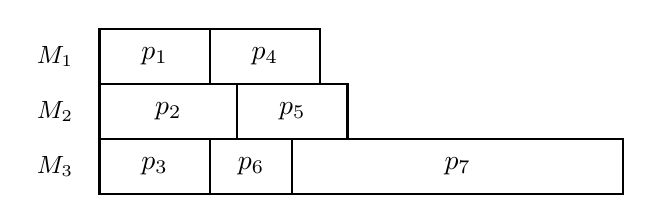
\begin{tikzpicture}[
    x=0.7cm,
    y=0.7cm,
    job/.style={
        draw,
        thick,
        fill=white,
        font=\small
    },
    machine/.style={font=\small}
]

% Displayed machine rows
\machinerow{1}{1}
\machinerow{2}{2}
\machinerow{3}{3}


% Edit the second schedule here.

\jobblock{1}{0}{2}{p_1}
\jobblock{1}{2}{2}{p_4}



\jobblock{2}{0}{2.5}{p_2}
\jobblock{2}{2.5}{2}{p_5}


\jobblock{3}{0}{2}{p_3}
\jobblock{3}{2}{1.5}{p_6}
\jobblock{3}{3.5}{6}{p_7}

\end{tikzpicture}
}

\DeclareMathOperator*{\supremum}{sup}

\begin{document}

\title{m=3, two jobs zero}
\author{}
\date{}
\maketitle

\section{Problem Introduction} 

\begin{lemma}[m=3]

    The approximation ratio of the $\mathrm{WSPT}$-rule for $3||\sum_{j} w_j C^{\alpha}_j$ is

   \[
\lambda_{\alpha}
=
\begin{cases}
1+
\frac{2}{\sqrt{\alpha(16+49\alpha)}+3\alpha} & \alpha\in (0,\frac12],\\[1.2ex]
\infty,
& \alpha=0.
\end{cases}
\]
\end{lemma}


The proof can be found in the Appendix ...

\begin{proof}
We know, from Singleton Job and Job Number bound, that we must only consider instances
with $n\le 3m-2=7$ jobs. Furthermore, we know that there is a singleton in $\sigma^*(I)$. 
The remaining instances can be expressed as follows: 

Let
\[
0\le \alpha\le \frac12 \quad\text{and}\quad
p_1,p_2,p_3,p_4,p_5,p_6,p_7>0.
\]
Set
\[
S:=p_1^2+p_2^2+p_3^2+p_4^2+p_5^2+p_6^2+p_7^2.
\]

The structural results... 
make it possible for us to express $\lambda_{\alpha}$ explicitly.

\[
\lambda_{\alpha}(I)
=
\frac{
(p_1+p_4)^2+(p_2+p_5)^2+(p_3+p_6+p_7)^2+(2\alpha-1)S
}{
(p_1+p_2+p_3)^2+(p_4+p_5+p_6)^2+p_7^2+(2\alpha-1)S
}
\]
subject to
\begin{align}
p_1+p_2+p_3&\ge p_4+p_5,
    \label{con:m3-load-123}\\
p_4+p_5+p_6&\ge p_1+p_2,
    \label{con:m3-load-456}\\
p_7&\ge p_1+p_2,
    \label{con:m3-p7-12}\\
p_7&\ge p_4+p_5,
    \label{con:m3-p7-45}\\
p_1+p_4&\ge p_3+p_6,
    \label{con:m3-p14-36}\\
p_2+p_5&\ge p_3+p_6,
    \label{con:m3-p25-36}\\
p_1+p_4&\ge p_2,
    \label{con:m3-p14-2}\\
p_2+p_5&\ge p_1,
    \label{con:m3-p25-1}\\
p_3+p_6+p_7&\ge p_1,
    \label{con:m3-p367-1}\\
p_3+p_6+p_7&\ge p_2.
    \label{con:m3-p367-2}
\end{align}

Where equations \eqref{con:m3-load-123} - \eqref{con:m3-p7-45} are sufficient conditions for 
$\sigma^{*}(I)$ to be list schedule, and \eqref{con:m3-p14-36} - \eqref{con:m3-p367-2} are sufficient 
for $\sigma^{W}(I)$ to be list schedule.


\begin{figure}[htbp]
\centering
\setlength{\fboxsep}{6pt}
\fbox{%
\begin{minipage}{0.94\textwidth}
    \begin{minipage}[t]{0.47\linewidth}
        \centering
        \scalebox{0.8}{\schedulethreeone}
        \par\smallskip
        \small(a) \(\sigma^{*}(I_1)\)
    \end{minipage}
    \hfill
    \begin{minipage}[t]{0.47\linewidth}
        \centering
        \scalebox{0.8}{\schedulethreetwo}
        \par\smallskip
        \small(b) \(\sigma^{W}(I_1)\)
    \end{minipage}
\end{minipage}%
}
\caption{Schedules for case (1)}
\label{figure-schedulecaseone}
\end{figure}


We will normalize the problem by setting
$p_7=1$
but keep $p_7$ as is for the moment for better readability of our calculations.

Constraints \eqref{con:m3-p367-1} and \eqref{con:m3-p367-2} are redundant. Indeed, since
\[
p_7\ge p_1+p_2
\]
and \(p_1,p_2>0\), we have \(p_7\ge p_1\) and \(p_7\ge p_2\). Hence
\[
p_3+p_6+p_7\ge p_1,\qquad p_3+p_6+p_7\ge p_2
\]
hold automatically.



Define
\[
L:=p_1p_2+p_1p_3+p_2p_3+p_4p_5+p_4p_6+p_5p_6
\quad \text{and}\quad
Q:=p_1p_4+p_2p_5+p_3p_6+p_7(p_3+p_6).
\]
Expanding the denominator of $\lambda_{\alpha}(I)$ gives
\[
\begin{aligned}
& (p_1+p_2+p_3)^2+(p_4+p_5+p_6)^2+p_7^2+(2\alpha-1)S\\
&=
2\alpha S+2(p_1p_2+p_1p_3+p_2p_3+p_4p_5+p_4p_6+p_5p_6)\\
&=
2(\alpha S+L).
\end{aligned}
\]
Similarly for the numerator,
\[
\begin{aligned}
& (p_1+p_4)^2+(p_2+p_5)^2+(p_3+p_6+p_7)^2+(2\alpha-1)S\\
&=
2\alpha S+2(p_1p_4+p_2p_5+p_3p_6+p_7(p_3+p_6))\\
&=
2(\alpha S+Q).
\end{aligned}
\]
Thus
\[
\lambda_{\alpha}(I)
=
\frac{\alpha S+Q}{\alpha S+L}
=
1+\frac{Q-L}{\alpha S+L}.
\]
Therefore the problem is equivalent to maximizing
\[
\frac{Q-L}{\alpha S+L}.
\]

Only one term in \(Q\) involves \(p_7\), namely
\[
p_7(p_3+p_6).
\]
The denominator contains the compensating term
\[
\alpha p_7^2.
\]
Thus, making \(p_7\) large cannot make the ratio
arbitrarily large.

Let
\[
x=p_3+p_6.
\]
The constraints
\[
p_1+p_4\ge x,\qquad p_2+p_5\ge x
\]
say that the two sums \(p_1+p_4\) and \(p_2+p_5\) must each carry at least the
mass \(x\).  We do not set these inequalities tight at this point.
Instead, the next section derives the active boundary algebraically and
only then checks that any slack in these two inequalities lowers the
ratio.
The same applies to the constraint \(p_2+p_5\ge p_1\): it is not assumed
tight.  After \(p_1+p_4=p_2+p_5=x\) and \(p_3=p_6=x/2\) have been reduced to,
the remaining dependence is through \(y=p_1+p_2\), and the numerator
\[
p_7x-\frac74x^2+2xy-y^2
\]
is maximized at \(y=x\); the denominator then forces \(p_1p_2=0\), so on
the symmetric branch \(p_1=x,p_2=0,p_5=x\), giving \(p_2+p_5=p_1\).


We now record the algebraic reduction leading to the active boundary.

\begin{lemma}[Reduction to the active boundary]
For \(0<\alpha\le \frac12\),
\[
\frac{Q-L}{\alpha S+L}
\le
\sup_{t>0}
\frac{t-\frac34t^2}
{\alpha+\left(1+\frac52\alpha\right)t^2}.
\]
\end{lemma}

\begin{proof}
Introduce the sums
\[
u=p_1+p_4,\qquad v=p_2+p_5,\qquad x=p_3+p_6.
\]
The constraints include
\[
u\ge x,\qquad v\ge x.
\]
Also put
\[
m=p_1+p_2,\qquad n=p_4+p_5.
\]
The constraints
\[
p_7\ge p_1+p_2,\qquad p_7\ge p_4+p_5
\]
become
\[
p_7\ge m,\qquad p_7\ge n.
\]
Finally,
\[
p_1+p_4\ge p_2,\qquad p_2+p_5\ge p_1
\]
become
\[
u\ge p_2,\qquad v\ge p_1.
\]

For fixed \(p_7\) and \(x=p_3+p_6\), expanding \(Q-L\) in the variables
\(u,v,m,p_3\) gives
\[
\begin{aligned}
Q-L
={}&p_7x-p_3^2+p_3(u+v+x-2m)-m^2\\
&+m(u+v+x)-uv-x(u+v).
\end{aligned}
\]
As we set
\[
p_1+p_4=x,\qquad p_2+p_5=x,
\]
we can analyze the remaining constraint \(p_2+p_5\ge p_1\). Choose the
maximizing ``split''
\[
p_3=p_6=\frac{x}{2},
\]
which is the maximal feasible choice for fixed \(x\), since it maximizes
\(p_3p_6\) (numerator) and minimizes \(p_3^2+p_6^2\) (denominator).
Then
\[
p_4=x-p_1,\qquad p_5=x-p_2.
\]
Put
\[
y=p_1+p_2.
\]
Then inserting gives
\[
Q-L
=
p_7x-\frac74x^2+2xy-y^2.
\]
For fixed \(x\) and \(p_7\), this quadratic in \(y\) is maximized at
\[
y=x.
\]
This can be seen by differentiation.

Thus the maximizing point satisfies
\[
p_1+p_2=x.
\]
Here, the denominator is
\[
\alpha S+L
=
\alpha p_7^2
+\left(1+\frac52\alpha\right)x^2
+(2-4\alpha)p_1p_2.
\]
Since \(0<\alpha\le \frac12\), the coefficient \(2-4\alpha\) is
nonnegative. Hence the denominator is minimized by
\[
p_1p_2=0.
\]
Consequently, either
\[
(p_1,p_2)=(x,0)
\qquad\text{or}\qquad
(p_1,p_2)=(0,x).
\]
The two cases are symmetric. We choose the first one, which implies
\[
p_5=x,\qquad p_2+p_5=x=p_1.
\]
Thus, the constraint
\(p_2+p_5\ge p_1\) is tight.

Finally, we need to check that this does not benefit from slack in
\(u\ge x\) or \(v\ge x\). We write
\[
u=x+r,\qquad v=x+s,\qquad r,s\ge0.
\]
This gives
\[
(p_1,p_2,p_3,p_4,p_5,p_6,p_7)
=
\left(x,s,\frac{x}{2},r,x,\frac{x}{2},p_7\right),
\]
so that
\[
p_1+p_4=x+r,\qquad
p_2+p_5=x+s,\qquad
p_3+p_6=x.
\]
For this family the excess numerator is
\[
Q-L
=
p_7x-\frac34x^2-\frac{x}{2}(r+s),
\]
whereas the denominator is
\[
\alpha S+L
=
\alpha p_7^2
+\left(1+\frac52\alpha\right)x^2
+\frac{3x}{2}(r+s)
+\alpha(r^2+s^2).
\]
Thus every positive slack \(r\) or \(s\) subtracts from the numerator
and adds to the denominator. Consequently, for fixed \(x\) and \(p_7\),
the largest value in this slack family is attained at
\[
r=s=0.
\]

Substituting the active equalities gives
\[
(p_1,p_2,p_3,p_4,p_5,p_6,p_7)
=
\left(x,0,\frac{x}{2},0,x,\frac{x}{2},p_7\right).
\]
We normalize \(p_7\) to get
\[
\left(t,0,\frac{t}{2},0,t,\frac{t}{2},1\right).
\]
On this boundary,
\[
Q-L=t-\frac34t^2
\]
and
\[
\alpha S+L
=
\alpha+\left(1+\frac52\alpha\right)t^2.
\]
Therefore every feasible point is bounded above by the one-variable
problem
\[
\sup_{t>0}
\frac{t-\frac34t^2}
{\alpha+\left(1+\frac52\alpha\right)t^2}.
\]
\end{proof}
\noindent
We continue by maximzing the one-variable function $f_{\alpha}$
Define
\[
f_\alpha(t)
=
\frac{t-\frac34t^2}{\alpha+\left(1+\frac52\alpha\right)t^2},
\qquad t>0.
\]
Set
\[
\beta=1+\frac52\alpha.
\]
Then
\[
f_\alpha(t)=\frac{t-\frac34t^2}{\alpha+\beta t^2}.
\]
Differentiate:
\[
f_\alpha'(t)
=
\frac{
\left(1-\frac32t\right)(\alpha+\beta t^2)
-
\left(t-\frac34t^2\right)(2\beta t)
}{
(\alpha+\beta t^2)^2
}.
\]
The numerator simplifies to
\[
\alpha-\frac32\alpha t-\beta t^2.
\]
Thus the critical point satisfies
\[
\beta t^2+\frac32\alpha t-\alpha=0.
\]
The positive root is
\[
t_\alpha
=
\frac{
-\frac32\alpha+\sqrt{\frac94\alpha^2+4\alpha\beta}
}{
2\beta
}.
\]
Since
\[
\beta=1+\frac52\alpha,
\]
we have
\[
\frac94\alpha^2+4\alpha\beta
=
4\alpha+\frac{49}{4}\alpha^2
=
\frac14\alpha(16+49\alpha).
\]
Therefore
\[
t_\alpha
=
\frac{\sqrt{\alpha(16+49\alpha)}-3\alpha}{4+10\alpha}.
\]

So the supremum over the reduced one-variable problem is

\[
\lambda_\alpha(t_\alpha)
= 1+
\frac{2}{\sqrt{\alpha(16+49\alpha)}+3\alpha}.
\]


The maximizing boundary point is only infeasible since in this instance we enfore 
there to be seven nonzero jobs. 
Therefore the expression above is only a supremum which can be approached by the family

\[
\left(
t_\alpha,\varepsilon,\frac{t_\alpha}{2},
\varepsilon,t_\alpha,\frac{t_\alpha}{2},1
\right)
\]
and $\varepsilon \rightarrow 0$.


Indeed though, taking the limit and deleting all jobs with processing time zero leaves us with a 
feasible instance that achieves the established $\lambda$-bound.
\[
\left(
t_\alpha,\frac{t_\alpha}{2},t_\alpha,\frac{t_\alpha}{2},1
\right).
\]

\begin{figure}[htbp]
\centering
\setlength{\fboxsep}{6pt}
\fbox{%
\begin{minipage}{0.94\textwidth}
    \begin{minipage}[t]{0.47\linewidth}
        \centering
        \scalebox{0.8}{\schedulethreemaxone}
        \par\smallskip
        \small(a) \(\sigma^{*}(I_1)\)
    \end{minipage}
    \hfill
    \begin{minipage}[t]{0.47\linewidth}
        \centering
        \scalebox{0.8}{\schedulethreemaxtwo}
        \par\smallskip
        \small(b) \(\sigma^{W}(I_1)\)
    \end{minipage}
\end{minipage}%
}
\caption{Maximzing Schedule}
\label{figure-sometjing}
\end{figure}
\end{proof}
\end{document}
